\documentclass[a4paper, 11pt]{article}
\usepackage[T1]{fontenc}
\usepackage[portuguese]{babel}
\usepackage[utf8]{inputenc}
\usepackage[margin=2cm,includefoot,includehead,footskip=30pt]{geometry}

\usepackage{graphicx}
\graphicspath{ {imagens/} }
\usepackage{bold-extra}
\usepackage{epstopdf}
\usepackage{float}
\usepackage{scalerel}
\usepackage{enumerate}
\usepackage{indentfirst}
\usepackage{cleveref}
\usepackage{amssymb}
\usepackage{listings}
\usepackage{color}
\usepackage{imakeidx}
\usepackage{enumitem}
\newcommand\showdiv[1]{\overline{\smash{\hstretch{.5}{)}\mkern-3.2mu\hstretch{.5}{)}}#1}}
\newcommand\ph[1]{\textcolor{white}{#1}}
\usepackage{upgreek}

\addto\captionsportuguese{
  \renewcommand{\contentsname}%
    {Índice}%
}

% ----- Cabeçalho e rodapé -----
\usepackage{fancyhdr}
\fancyhf{}

\renewcommand{\headrulewidth}{0.5pt}
\renewcommand{\footrulewidth}{0.5pt}

\rhead{Wordmorph}
\lhead{Algoritmos e Estruturas de Dados}
\rfoot{Página \thepage}
\lfoot{\small Engenharia Electrotécnica e de Computadores - IST}


\usepackage{pdfpages}

\begin{document}

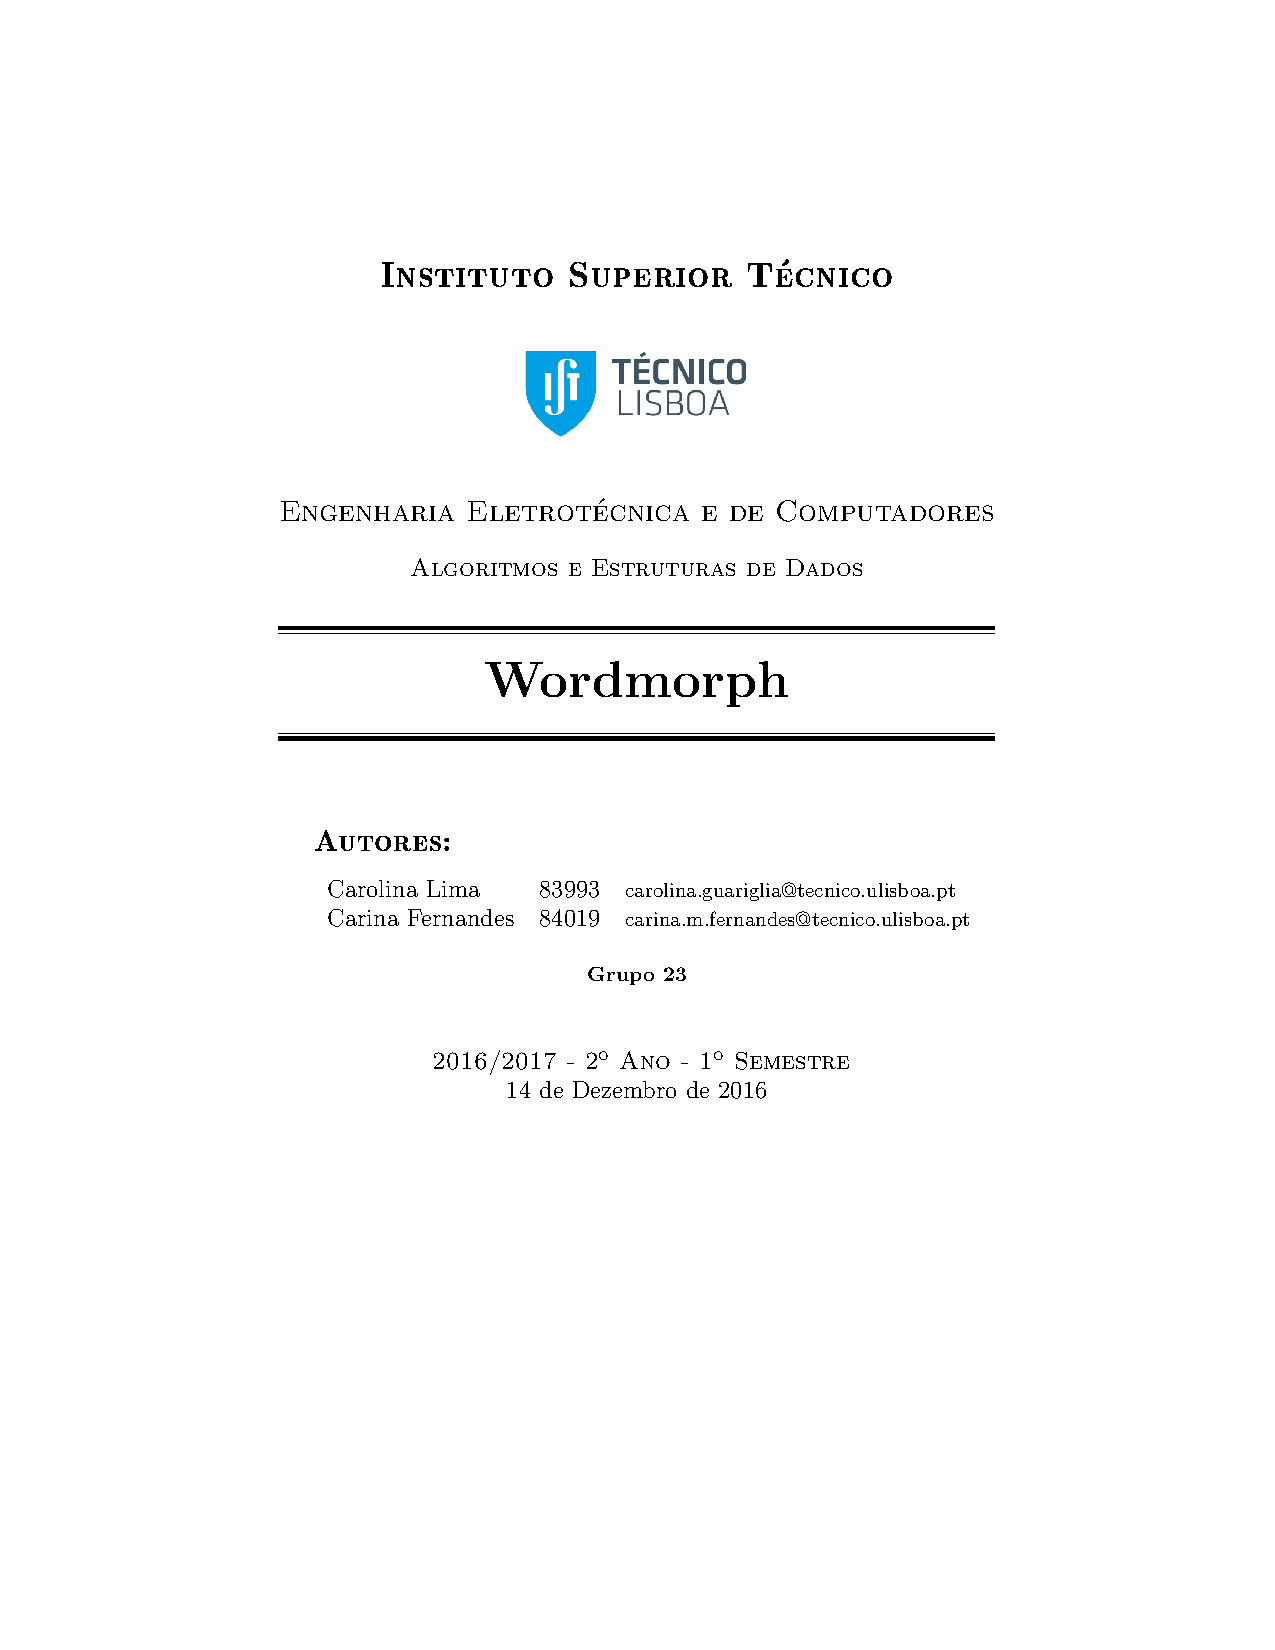
\includepdf[pages={1}]{capa/capa.pdf}

\pagestyle{fancy}
\tableofcontents
\newpage

\section{Descrição do problema}
    \par O problema enunciado consiste na procura de caminhos entre palavras. Estes caminhos são, na verdade, uma sequência de palavras de tamanho igual no qual cada palavra se obtêm mudando uma ou mais letras da palavra anterior, até chegar à palavra desejada. Para além disso, todas as palavras pertencentes ao caminho têm obrigatoriamente de pertencer a um dicionário. Dicionário é definido neste caso como uma lista de palavras, que não têm obrigatoriamente de ser todas do mesmo tamanho.
    \par Como é possível a existência de vários caminhos, distingue-se cada passo do caminho pelo número de caracteres que são mudados. No fim, os custos dos caminhos somam-se para chegar ao custo final. Por exemplo, um passo no qual se mude um caracter têm o custo de $1^1$, um passo em que se mudam dois caracteres têm um custo de $2^2$, e assim sucessivamente.
    \par O objectivo final deste projecto é, dado duas palavras e o número máximo de trocas que se podem efectuar em cada passo, retornar o caminho de menor custo entre essas duas palavras.
    
\section{Abordagem do problema}
    \par Para resolver o problema, decidiu-se dividi-lo nas seguintes partes: guardar as palavras do dicionário e procurar o caminho propriamente dito. Chegou-se então à conclusão de que seria necessário guardar as palavras do dicionário num local que fosse facilmente acessível, e que não seria necessário guardar todas as palavras, apenas as relevantes, tal como não é necessário fazer todos os grafos.
\subsection{Procura do caminho de menor custo}
    \par A escolha óbvia para resolver este problema foi recorrer ao algorítmo de Dijkstra, que procura o caminho mais curto entre dois vértices de um dado grafo desde que nenhuma das arestas do mesmo tenha peso negativo, o que é o caso deste problema. Para podermos utilizar então o algorítmo, chegou-se então à conclusão que é necessária a criação de um grafo representado por listas de adjacências (o algorítmo não é igual para matrizes de adjacência).
    
\section{Implementação do programa}
    \par Dividiu-se então o programa em três partes distintas: uma parte referente às estruturas de dados, uma parte que se relaciona diretamente com o problema a resolver, e por fim todas as restantes operações que não pertencem a nenhum dos anteriores grupos. No código, estas partes equivalem aos ficheiros datastructs.c, words.c e utils.c respectivamente.
    \par Para evitar alocações de memória desnecessárias, percorrem-se todas as linhas do ficheiro de dicionário duas vezes. Uma para contar o número de palavras que existem de cada tamanho de palavra, outra para copiar as palavras do ficheiro para a matriz que representa o dicionário, cujo tamanho é alocado baseando-se no número obtido anteriormente. Assumiu-se que nunca existiriam palavras de mais de cem letras.
    \par Como mencionado na secção anterior, rapidamente chegou-se à conclusão de que é desnecessário criar grafos que não vão ser utilizados. Por isso, também percorre-se uma vez pelo ficheiro de problemas sem os começar a resolver, para saber que tamanhos de palavras existem no ficheiro, e qual número máximo de caracteres que mudam entre duas palavras do caminho.
    
\subsection{Descrição das estruturas de dados}
    \par Como referido acima, foi claro que seria necessária a criação de uma lista de adjacências, então foi implementada uma lista genérica. Esta é definida usando $void *$ (definido em datastructs.h, e a partir daqui referido como Item), para os quais se pode passar qualquer ponteiro, assegurando a generalidade da implementação.
    \par As listas definidas foram então utilizadas na definição do grafo pois este é implementado usando uma lista de adjacências. Os grafos foram definidos de forma genérica, com um reparo - a implementação dos dados usados na lista estão visíveis ao cliente. Todos os novos elementos desta lista são inseridos na primeira posição (head).
    \par Como terá de existir um grafo para cada tamanho de palavras, decidiu-se usar um vetor para guardá-los no qual o índice corresponde ao tamanho das palavras representadas no grafo (i.e. all{\_}arrays[3] contêm o grafo das palavras de tamanho 3).
    \par Por fim, a descrição do algorítmo de Dijkstra requer um acervo, também este definida de forma genérica no código. Neste caso, o acervo foi implementado usando uma fila prioritária, que por sua vez foi implementada usando um vector. Este vector tem um tamanho fixo, definido na sua incialização, mas usou-se outra vaŕiavel (q$\rightarrow$first) para que exista um ``vector virtual''  dentro do vector maior. Outra das variáveis que foi útil foi um vector indexado por vértices que diz onde o vértice está na heap (q$\rightarrow$vert{\_}pos), que evita que se tenha de fazer procura linear cada vez que se quer encontrar um vértice na heap.
    
\subsection{Descrição dos algoritmos}
    \par Claramente, o algorítmo crucial ao programa foi o algoritmo de Dijkstra, usando a variação que encontra o caminho mais curto entre dois vértices e não a que encontra o caminho mais curto entre um vértice e todos os outros vértices do grafo, ou seja, parando quando o elemento que sai da heap é o vértice a que se quer chegar.
    
\section{Subsistemas funcionais}
    \par Como já referido, existem três subsistemas funcionais:
    \begin{description}[align=left]
       \item[datastructs.c] Implementa os três tipos de dados essenciais - listas ligadas, grafos e acervos. Inclui as funções requiridas por cada tipo de dados, como a inicialização, libertação de memória e funções de interface para que o cliente possa interagir com as estruturas.
       \item[utils.c] Funções variadas que não fariam sentido estar noutro ficheiro. Tem funções que lidam com a abertura de ficheiros, comparações, e a implementação do algorítmo de Dijkstra.
       \item[words.c] Encontra-se tudo que se relaciona diretamente com a resolução do problema, como por exemplo a determinação da maior permutação e a leitura das palavras dos ficheiros de dicionário e problemas.
    \end{description}

\section{Complexidade do programa}
    \par Examinando o programa, chega-se à conclusão de que existem duas grandes partes que contribuem para a complexidade. Em ambos os casos, $v$ representa o número total de palavras com o mesmo tamanho e $e$ representa o número de ligações que existem entre palavras.
    \begin{description}[align=left]
        \item[Criação de grafo] Para inserir todas as palavras no grafo, é necessário comparar todas as palavras duas a duas. No código, como para cada palavra do dicionário só é necessário comparar as palavras anteriores a esta, o que acontece é $1 + 2 + 3 + ... + v = \frac{v^2}{2} + \frac{v}{2}$, que é majorado por $v^2$ concluindo-se então que a complexidade será $O(v^2)$.
        \par Em termos de memória, a complexidade será de $O(e^2)$, visto que numa lista de adjacências de um grafo não direccionado uma ligação é reperesentada por dois nós.
        \item[Algorítmo de Dijkstra] No caso do problema a resolver, observa-se que o grafo que representa as ligações é um grafo esparso (menos do que $|v^2|$ ligações). Assim, esta implementação do algorítmo de Dijkstra, usando uma lista de adjacências e um acervo, corre em $\Uptheta((|e| + |v|)log(|v|))$, como há uma estrutura de dados auxiliar que indica aonde está cada vértice na heap, fazendo com que a procura seja $O(1)$.
    \end{description}

\section{Análise do programa}
    \par Na supefície, o problema é simples - no entanto é necessária alguma cautela para alguns casos limite e para alguns descuidos que podem aumentar e muito o tempo de execução do problema. Um destes descuidos foi a procura de um determinado vértice dentro da \textit{heap} - a abordagem \textit{naïve} utilizada inicialmente tinha complexidade $O(n)$, o que considando as vezes que era necessário descobrir o vértice, ``estragava'' a rapidez do algorítmo de Dijkstra.
    \par Outro problema, que foi mais trivial de resolver, foi o facto de que não foram antecipados certos tipos de problemas, nomeadamente que a palavra de partida fosse igual à palavra de chegada e que a diferença entre as palavras fosse apenas de uma letra.

\section{Exemplo}
    \par Considerando como exemplo um ficheiro de problemas com:
        \begin{center}
        \texttt{massa pasta 3 \\
        pasta pasta 1 \\
        pasta parte 2 \\
        }
        \end{center}
        
    \par E considerando que um dicionário um ficheiro com palavras não acentuadas, sem hífen, separadas por espaços ou \textit{newlines} e que inclui todas as palavras que se encontram no ficheiro de problemas, como por exemplo: 
        \begin{center}
        \texttt{juiz largo \\
        massa parte \\
        pasta rei \\
        ...}
        \end{center}
        
    \par Então, os passos que se efectuam para resolver o ficheiro de problemas enunciado são:
    
    \begin{enumerate}[align=left]
        \item Lê-se o ficheiro de problemas de forma a identificar o número máximo de mutações entre palavras de um determinado tamanho, ignorando casos triviais como duas palavras iguais ou duas palavras que apenas diferem em uma letra.
        \item Guarda-se as palavras com tamanhos relevantes à resolução numa matriz.
    \end{enumerate}

\section{Bibliografia}


\end{document}
